% example.tex
\documentclass[dvisvgm]{standalone}

\usepackage{amsmath}
\usepackage[usenames,dvipsnames]{xcolor}
\usepackage{amsmath}
\usepackage{tikz}
\usetikzlibrary {angles,
                 arrows.meta,
                 calc,
                 positioning,
                 shapes.geometric}

 \tikzset{
        proc/.style={draw, align= left, rectangle,  
        minimum width=7.5cm, minimum height=3cm},
        io/.style={trapezium, trapezium left angle=70, trapezium right
                   angle=110, draw, text width=8em, %minimum width=2cm, 
                   %minimum height=1cm
                   },
        test/.style={base, diamond, aspect=2,
                     %text width=5em
                     },
        term/.style={proc, rounded corners},
        myarrow/.style={-Stealth, line width=0.25mm},
 }



\begin{document}
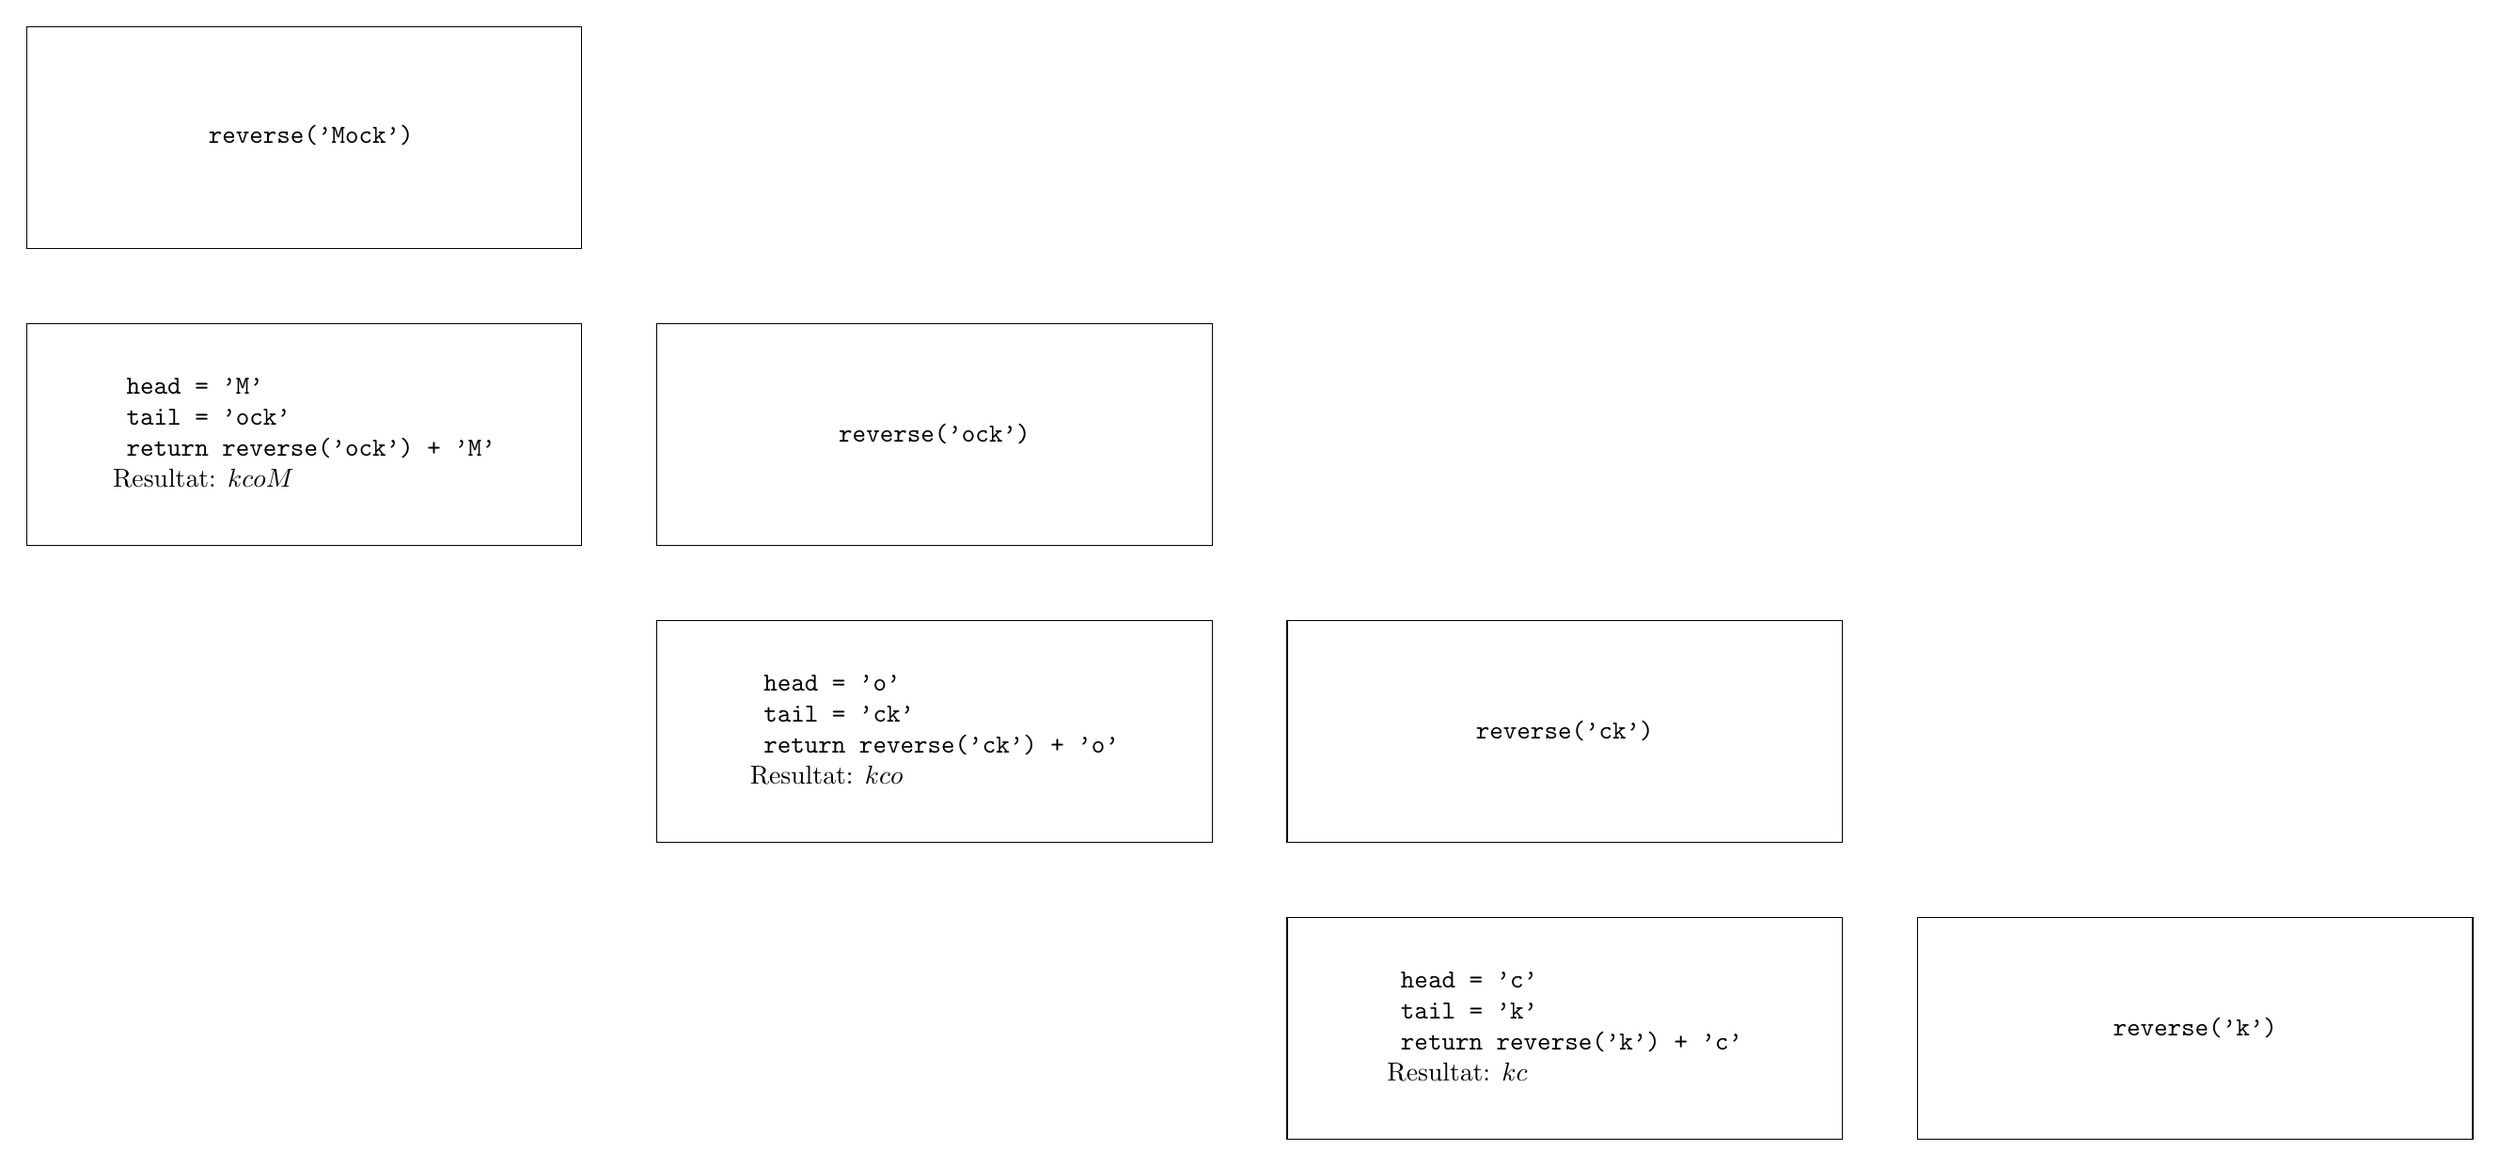
\begin{tikzpicture}
    \node[draw, proc] (input)
    {\begin{tabular}{l}
        \verb| reverse('Mock') |\\
    \end{tabular}};

    \node[draw, proc, below = of input](level0) 
    {\begin{tabular}{l}
        \verb| head = 'M' |\\
        \verb| tail = 'ock' |\\
        \verb| return reverse('ock') + 'M' |\\
        Resultat: $kcoM$\\
    \end{tabular}};
   
    \node[draw, proc, right= of level0] (call1) {\verb| reverse('ock') |};

    \node[draw, proc, below = of call1](level1) 
    {\begin{tabular}{l}
        \verb| head = 'o' |\\
        \verb| tail = 'ck' |\\
        \verb| return reverse('ck') + 'o' |\\
        Resultat: $kco$\\
    \end{tabular}};

    \node[draw, proc, right= of level1] (call2) {\verb| reverse('ck') |};

    \node[draw, proc, below = of call2](level2) 
    {\begin{tabular}{l}
        \verb| head = 'c' |\\
        \verb| tail = 'k' |\\
        \verb| return reverse('k') + 'c' |\\
        Resultat: $kc$\\
    \end{tabular}};

    \node[draw, proc, right= of level2] (call3) {\verb| reverse('k') |};

\end{tikzpicture}
\end{document}
